% !TEX root = ./article.tex

\documentclass{article}

\usepackage{mystyle}
\usepackage{myvars}



%-----------------------------

\begin{document}

	\maketitle % Insert title

	\thispagestyle{fancy} % All pages have headers and footers


%-----------------------------
%	ABSTRACT
%-----------------------------

	\begin{abstract}
		\noindent [TODO ]
	\end{abstract}

%-----------------------------
%	TEXT
%-----------------------------


	\section{Introducción}
	\label{sec:introducción}

		\paragraph{}
		[TODO]

		\subsection{Regresión Lineal Múltiple}

			\paragraph{}
			[TODO]



		\subsection{Regresión Logística}

			\paragraph{}
			[TODO]




	\section{Evaluación de resultados a partir de distintas cotas de error relativo para Regresión Lineal Múltiple}
	\label{sec:e1}

		\paragraph{}
		[TODO

		\begin{figure}
			\begin{center}
				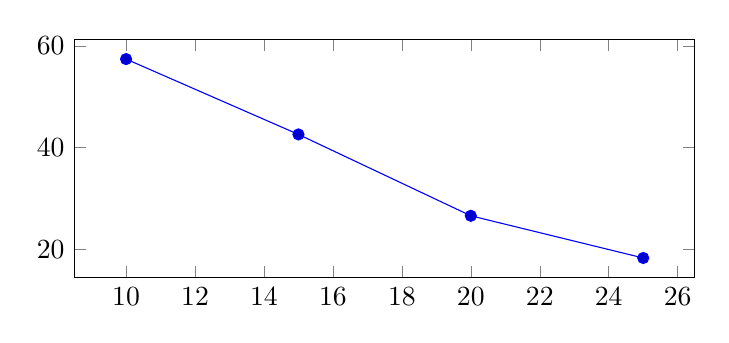
\begin{tikzpicture}
					\begin{axis}[
						% only scale the axis, not the axis including the ticks and labels
						scale only axis=true,
						% set `width' and `height' to the desired values
						width=0.65\textwidth,
						height=0.25\textwidth,
						]
						\addplot coordinates {
							(10,57.396)
							(15,42.604)
							(20,26.627)
							(25,18.343)
						};
					\end{axis}
				\end{tikzpicture}
			\end{center}
			\caption{[ TODO]}
			\label{plot:e1}
		\end{figure}

		\paragraph{}
		[TODO ]
		
		\begin{table}
			\centering
			\small
			\begin{tabu}{ | c | c | c | c | c | c | c | c | c | c | }
				\hline
				\multicolumn{5}{ | c | }{HoldOut 66\%/33\% --- Regresión --- Housing Dataset} \\ \hline
				\multirow{2}{*}{Datos}	& \multicolumn{4}{ c |}{Tasa de Error} \\ \cline{2-5}
																& \emph{Lineal 10\%} & \emph{Lineal 15\%} & \emph{Lineal 20\%} & \emph{Lineal 25\%}\\ \hline
				Entrenae						& $57.396\%$	 & $42.604\%$ & $26.627\%$ & $18.343\%$ \\
				\hline
			\end{tabu}
			\caption{[TODO ]}
			\label{table:e2}
		\end{table}

	\section{Comparación de resultados entre Regresión Logística y Regresión Lineal Múltiple}
	\label{sec:e2}

		\paragraph{}
		[TODO]


		\begin{figure}
			\begin{center}
				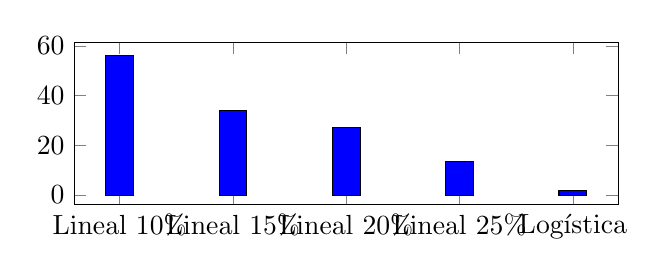
\begin{tikzpicture}
					\begin{axis}[
						symbolic x coords={Lineal 10\%,Lineal 15\%,Lineal 20\%,Lineal 25\%,Logística},
						width=0.7\textwidth,
						height=0.3\textwidth,
						xtick=data]
						\addplot[ybar, fill=blue] coordinates {
							(Lineal 10\%, 55.932)
							(Lineal 15\%, 33.898)
							(Lineal 20\%, 27.119)
							(Lineal 25\%, 13.559)
							(Logística, 1.6949)
						};
					\end{axis}
				\end{tikzpicture}
			\end{center}
			\caption{[TODO ]}
			\label{plot:e2}
		\end{figure}

		\paragraph{}
		[TODO ]

		\begin{table}
			\centering
			\small
			\begin{tabu}{ | c | c | c | c | c | c | c | c | c | c | }
				\hline
				\multicolumn{6}{ | c | }{HoldOut 66\%/33\% --- Regresión --- Wine Dataset} \\ \hline
				\multirow{2}{*}{Datos}	& \multicolumn{5}{ c |}{Tasa de Error} \\ \cline{2-6}
																& \emph{Lineal 10\%} & \emph{Lineal 15\%} & \emph{Lineal 20\%} & \emph{Lineal 25\%} & \emph{Logística}\\ \hline
				Entrenae						& $55.932\%$	 & $33.898\%$ & $27.119\%$ & $13.559\%$	& $1.6949\%$ \\
				\hline
			\end{tabu}
			\caption{[TODO ]}
			\label{table:e2}
		\end{table}



%-----------------------------
%	Bibliographic references
%-----------------------------
	\nocite{garciparedes:machine-learning-regression}
	\nocite{subject:taa}
	\nocite{tool:weka}
  \bibliographystyle{alpha}
  \bibliography{bib/misc}

\end{document}
